\documentclass[aps,pra,11pt,onecolumn,nofootinbib,tightenlines]{revtex4-2}

\usepackage{mathrsfs}
\usepackage{amsmath}
\usepackage{amsfonts}
\usepackage{amssymb}
\usepackage{amsthm}
\usepackage{tikz}
\usetikzlibrary{arrows.meta,positioning}
\usepackage{booktabs}
\usepackage[colorlinks=true,urlcolor=blue,citecolor=blue,linkcolor=blue]{hyperref}
\usepackage{xurl}
\usepackage{natbib}

\newcommand{\LeanDecl}[1]{\path{#1}}
\newcommand{\Formalized}{\textup{Formalized}}
\renewcommand{\thesection}{\arabic{section}}

\begin{document}

\title{Lean Formalization of the Parameter Classification for Conditional Entropies}

\begin{abstract}
This note records the Lean formalization of the necessary-and-sufficient
parameter classification for the concrete conditional-entropy candidates of
Refs.~\cite{rubboli2026complete,rubboli2026parametersConcise,
rubboli2026parametersFull}. It gives a compact dependency graph, a
statement-by-statement correspondence table, and the precise trust and scope
boundary. The presentation is deliberately theorem-facing: it separates the
public conclusions, their paper-level ingredients, and the proved reusable
infrastructure.
\end{abstract}

\author{Roberto Rubboli}
\noaffiliation
\author{Erkka Haapasalo}
\noaffiliation
\author{Marco Tomamichel}
\noaffiliation

\maketitle

\section{Lean correspondence}
\label{sec:lean-correspondence}

The formal development follows the mathematical proof in the concise and
full-detail companion papers. It covers the endpoint-aware R\'enyi parameter,
real-power and entropy differentiation, signed integration, common
discretization, the two-block, three-block, and Shannon localizers, exact
tropical stationarity, all sufficiency and necessity branches, and the
original finite semiring and conditionally mixing channel lift. The source is
available at
\url{https://github.com/robertorubboli/A-complete-characterization-of-conditional-entropies}
under the release tag \texttt{four-document-release-2026-08-25}.

Throughout this note, every numbered reference to a lemma, proposition, or
remark is the number in the full-details Sections~4 and~5 paper,
Ref.~\cite{rubboli2026parametersFull}. The concise companion,
Ref.~\cite{rubboli2026parametersConcise}, uses the identical statement order and
numbering, so the same label locates the corresponding concise statement.

There are two public conclusions. The declaration
\LeanDecl{mainClassification} says that, for every probability measure on the
compactified R\'enyi parameter space, monotonicity of each concrete candidate
is equivalent to its exact admissibility condition. Its only explicit argument
is the measure being classified; it has no auxiliary hypothesis. The closed
declaration \LeanDecl{allConditionalEntropyAxioms} proves nonnegativity,
zero-embedding invariance, tensor additivity, fair-bit normalization, and
embedded channel monotonicity for every admissible candidate. Neither theorem
assumes a project-specific axiom.

Figure~\ref{fig:lean-dependencies} shows the proof at theorem level. Arrows
point from a conclusion to ingredients used in its proof. Pale green boxes
are the two public conclusions, white boxes are paper-facing intermediate
results, pale blue boxes are reusable infrastructure that is itself proved in
Lean, and the dashed gray box is an upstream representation theorem cited from
Section~3 of Ref.~\cite{rubboli2026complete}. That gray result is needed only
for the statement that every abstract derivation has the displayed barycentric
form; it is not an axiom or hypothesis of either green Lean declaration.

\begin{figure}[htbp]
\centering
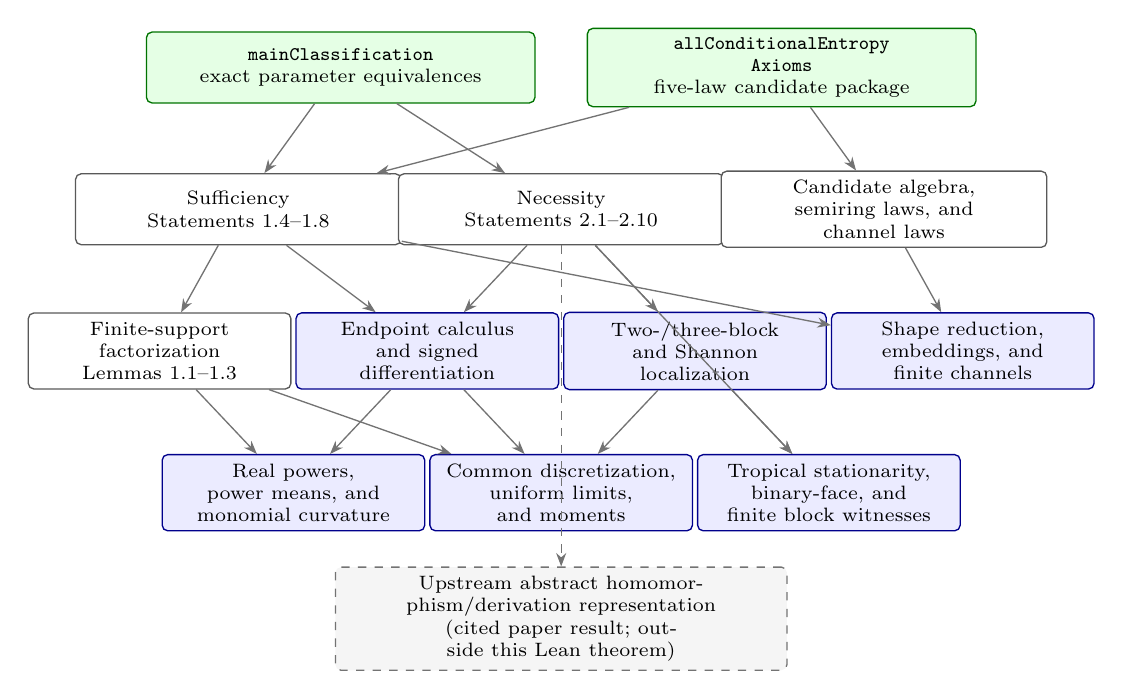
\begin{tikzpicture}[
  >=Stealth,
  every path/.style={draw=black!55,line width=.48pt,-{Stealth[length=1.7mm]}},
  final/.style={draw=green!45!black,fill=green!10,rounded corners=2pt,
    align=center,font=\scriptsize,text width=47mm,minimum height=9mm},
  paper/.style={draw=black!65,fill=white,rounded corners=2pt,
    align=center,font=\scriptsize,text width=39mm,minimum height=9mm},
  infra/.style={draw=blue!55!black,fill=blue!8,rounded corners=2pt,
    align=center,font=\scriptsize,text width=31mm,minimum height=9mm},
  papercompact/.style={draw=black!65,fill=white,rounded corners=2pt,
    align=center,font=\scriptsize,text width=31mm,minimum height=9mm},
  boundary/.style={draw=black!55,dashed,fill=black!4,rounded corners=2pt,
    align=center,font=\scriptsize,text width=55mm,minimum height=9mm}]

\node[final] (classification) at (-2.8,0)
  {\texttt{mainClassification}\\exact parameter equivalences};
\node[final] (laws) at (2.8,0)
  {\texttt{allConditionalEntropy}\\\texttt{Axioms}\\five-law candidate package};

\node[paper] (suff) at (-4.1,-1.8)
  {Sufficiency\\Statements~1.4--1.8};
\node[paper] (necess) at (0,-1.8)
  {Necessity\\Statements~2.1--2.10};
\node[paper] (candidate) at (4.1,-1.8)
  {Candidate algebra,\\semiring laws, and\\channel laws};

\node[papercompact] (finite) at (-5.1,-3.6)
  {Finite-support\\factorization\\Lemmas~1.1--1.3};
\node[infra] (endpoint) at (-1.7,-3.6)
  {Endpoint calculus\\and signed\\differentiation};
\node[infra] (local) at (1.7,-3.6)
  {Two-/three-block\\and Shannon\\localization};
\node[infra] (channel) at (5.1,-3.6)
  {Shape reduction,\\embeddings, and\\finite channels};

\node[infra] (powers) at (-3.4,-5.4)
  {Real powers,\\power means, and\\monomial curvature};
\node[infra] (disc) at (0,-5.4)
  {Common discretization,\\uniform limits,\\and moments};
\node[infra] (stationary) at (3.4,-5.4)
  {Tropical stationarity,\\binary-face, and\\finite block witnesses};

\node[boundary] (upstream) at (0,-7.0)
  {Upstream abstract homomorphism/derivation representation\\
   (cited paper result; outside this Lean theorem)};

\draw (classification) -- (suff);
\draw (classification) -- (necess);
\draw (laws) -- (suff);
\draw (laws) -- (candidate);
\draw (suff) -- (finite);
\draw (suff) -- (endpoint);
\draw (suff) -- (channel);
\draw (necess) -- (endpoint);
\draw (necess) -- (local);
\draw (necess) -- (stationary);
\draw (candidate) -- (channel);
\draw (finite) -- (powers);
\draw (finite) -- (disc);
\draw (endpoint) -- (powers);
\draw (endpoint) -- (disc);
\draw (local) -- (disc);
\draw (local) -- (stationary);
\draw[dashed] (necess) -- (upstream);
\end{tikzpicture}
\caption{Dependency graph for the Lean formalization. Every displayed
statement number is the number in the full-details Sections~4 and~5 paper,
Ref.~\cite{rubboli2026parametersFull}; the concise companion uses the same
numbering. Arrows point to proof ingredients. Color records proof role, not
confidence: green means public conclusion, blue means internally proved
infrastructure, white means a paper-facing result, and dashed gray marks the
explicitly excluded upstream representation theorem.}
\label{fig:lean-dependencies}
\end{figure}

Table~\ref{tab:lean-correspondence} follows, statement by statement, the
numbering of the full-details Sections~4 and~5 paper,
Ref.~\cite{rubboli2026parametersFull}. The concise companion uses the same
numbers. All Lean names are in the namespace \LeanDecl{ConditionalEntropy}. A
split API means that one manuscript statement is intentionally proved by
several smaller declarations. The last row is worded differently because
Proposition~2.10 combines the formalized parameter restriction with the
upstream representation theorem identified above.

\renewcommand{\arraystretch}{1.12}
\begin{table}[htbp]
\centering
\small
\caption{Statement-by-statement correspondence. All lemma, proposition, and
remark numbers are those of the full-details Sections~4 and~5 paper,
Ref.~\cite{rubboli2026parametersFull}; the concise companion uses the same
numbering.}
\label{tab:lean-correspondence}
\begin{tabular}{p{0.25\textwidth}p{0.49\textwidth}p{0.18\textwidth}}
\toprule
Manuscript statement & Lean declaration & Status\\
\midrule
Lemma~1.1: power-mean curvature &
\LeanDecl{finiteHolder}; \LeanDecl{powerCurvature};
\LeanDecl{parameterPowerCurvature} & \Formalized\\
\addlinespace
Lemma~1.2: monomial curvature &
\LeanDecl{affineMonomialCurvaturePackage} & \Formalized\\
\addlinespace
Lemma~1.3: finite-support sufficiency &
\LeanDecl{finiteSufficiency} & \Formalized\\
\addlinespace
Proposition~1.4: general temperate sufficiency &
\LeanDecl{generalSufficiency}; \LeanDecl{finiteTSufficiency} &
\Formalized\ (split API)\\
\addlinespace
Proposition~1.5: negative-tropical sufficiency &
\LeanDecl{negativeTropicalSufficiency} & \Formalized\\
\addlinespace
Proposition~1.6: positive-tropical sufficiency &
\LeanDecl{positiveTropicalComponent};
\LeanDecl{positiveTropicalSufficiency} & \Formalized\ (split API)\\
\bottomrule
\end{tabular}
\end{table}

\begin{table}[htbp]
\centering
\small
\textbf{Table~\ref{tab:lean-correspondence} (continued; statement numbers are
from the full-details Sections~4 and~5 paper).}\par\smallskip
\begin{tabular}{p{0.25\textwidth}p{0.49\textwidth}p{0.18\textwidth}}
\toprule
Manuscript statement & Lean declaration & Status\\
\midrule
Remark~1.7: exact tropical endpoint families &
Tropical fields of \LeanDecl{mainClassification} &
\Formalized\ (split API)\\
\addlinespace
Proposition~1.8: derivation sufficiency &
\LeanDecl{derivationSufficiency} & \Formalized\\
\addlinespace
Proposition~2.1: positive necessity &
\LeanDecl{positiveNecessity};
\LeanDecl{positiveTemperateProbabilityNecessity} &
\Formalized\ (split API)\\
\addlinespace
Proposition~2.2: negative Shannon atom with upper support &
\LeanDecl{negativeShannonObstruction} & \Formalized\\
\addlinespace
Proposition~2.3: truncated exceptional-moment bound &
\LeanDecl{truncatedMoment};
\LeanDecl{exceptionalUpperMeasurePackage};
\LeanDecl{MLower_le_of_truncated_difference} &
\Formalized\ (split API)\\
\bottomrule
\end{tabular}
\end{table}

\begin{table}[htbp]
\centering
\small
\textbf{Table~\ref{tab:lean-correspondence} (continued; statement numbers are
from the full-details Sections~4 and~5 paper).}\par\smallskip
\begin{tabular}{p{0.25\textwidth}p{0.49\textwidth}p{0.18\textwidth}}
\toprule
Manuscript statement & Lean declaration & Status\\
\midrule
Remark~2.4: homogeneity and channel lift &
\LeanDecl{columnPhi_posHomOne};
\LeanDecl{columnDeriv_posHomOne};
\LeanDecl{conditionalSemiringOfJointProb_le};
\LeanDecl{embeddingLift} & \Formalized\ (split API)\\
\addlinespace
Remark~2.5: compensated two-column witness &
\LeanDecl{normalizedTwoColumn};
\LeanDecl{normalizedTwoColumn_column_zero};
\LeanDecl{normalizedTwoColumn_column_one};
\LeanDecl{mergeTwoChannel_output_column};
\LeanDecl{sum_normalizedTwoColumn} & \Formalized\ (split API)\\
\addlinespace
Proposition~2.6: at most one upper support point &
\LeanDecl{oneUpperPoint};
\LeanDecl{negativeTemperateNecessity_of_atom_zero} &
\Formalized\ (split API)\\
\bottomrule
\end{tabular}
\end{table}

\begin{table}[htbp]
\centering
\small
\textbf{Table~\ref{tab:lean-correspondence} (continued; statement numbers are
from the full-details Sections~4 and~5 paper).}\par\smallskip
\begin{tabular}{p{0.25\textwidth}p{0.49\textwidth}p{0.18\textwidth}}
\toprule
Manuscript statement & Lean declaration & Status\\
\midrule
Proposition~2.7: negative-tropical necessity &
\LeanDecl{negativeTropicalUpperAtomZero};
\LeanDecl{twoUpperSupportPointsTropicalObstruction};
\LeanDecl{tropicalTruncatedMoment_of_exceptional};
\LeanDecl{negativeTropicalNecessity} &
\Formalized\ (split API)\\
\addlinespace
Proposition~2.8: positive-tropical necessity &
\LeanDecl{sameSupportDecomposition};
\LeanDecl{probabilityEqDiracZero};
\LeanDecl{positiveTropicalNecessity} &
\Formalized\ (split API)\\
\addlinespace
Proposition~2.9: derivation necessity &
\LeanDecl{derivationNecessity} & \Formalized\\
\addlinespace
Proposition~2.10: represented derivations &
\LeanDecl{derivationSufficiency};
\LeanDecl{derivationNecessity}; derivation field of
\LeanDecl{mainClassification} &
Range proved; representation cited\\
\bottomrule
\end{tabular}
\end{table}

The table records the human-facing correspondence. The repository also keeps
the complete implementation ledger with 152 source-ordered rows, together with
the declaration index and editable module-level dependency graph. Those longer
audits are kept out of this note so that the main proof route remains readable.

\subsection{Trust boundary and reproducibility}

The project is pinned to Lean~4.32.2 and Mathlib~4.32.2. The release source
contains no \texttt{sorry}, \texttt{admit}, project-defined \texttt{axiom}, or
project-defined \texttt{opaque} declaration. The final declarations contain no
unproved project hypothesis. Lean's standard logical foundations, including
classical choice, propositional extensionality, and quotient soundness, remain
part of the ordinary trusted base.

The single command
\begin{verbatim}
powershell -File scripts/check.ps1
\end{verbatim}
runs the forbidden-token scan, a warning-as-error build of the integrated
\LeanDecl{CompleteCharacterization} target, the axiom audit, and the exact
correspondence audit. The formalization proves the classification and law
package for the four concrete candidate families. The upstream representation
of every abstract homomorphism or derivation, the later barycentric
classification of every abstract conditional entropy, and the large-sample,
catalytic, and application results remain results of
Ref.~\cite{rubboli2026complete}, not hidden assumptions of the Lean terminal
theorems.

\bibliographystyle{ultimate}
\renewcommand{\bibfont}{\footnotesize}
\bibliography{bibliography}

\end{document}
